The alignment of stars that led, in 2011/2012, to the concept of a $\sim$\,100\,km electron-positron collider in the same tunnel as a future 100\,TeV proton-proton collider in the Geneva basin and, in 2020, to the update of the European Strategy for Particle Physics (ESPPU) endorsing the FCC feasibility study as a top priority for CERN and its international partners, has presented the global HEP community with a unique and exceptional opportunity to advance the field. 
After almost five years of Feasibility Study performed by a worldwide consortium of scientists and engineers, the particle physicists ---including the early-career contingent--- are now steadily coalescing around the initial-stage machine (FCC-ee) as the first priority for a post-LHC collider at CERN. 

The FCC-ee offers ideal conditions (high luminosity, centre-of-mass energy calibration, possibly mono\-chromatisation, and moderate beam-induced backgrounds) for the intensity-frontier study of the four heaviest particles of the Standard Model, accumulating enormous samples ($6\times 10^{12}$ \PZ bosons at 88--94\,GeV, $5 \times 10^8$ \PW bosons at and above 157\,GeV, $2.8 \times 10^6$ Higgs bosons at and above 240\,GeV, and $4 \times 10^6$ top quarks at and above 340\,GeV) in only a few years of operation at each energy point. With a wealth of opportunities for precision electroweak, QCD, flavour, and Higgs measurements, searches for rare or forbidden processes, and the possible discovery of feebly coupled particles, \mbox{FCC-ee} is sensitive to essentially any kind of new physics from a few GeV up to scales of 10 to 100\,TeV, over an extremely broad range of couplings. These studies may help address the most profound questions of particle physics today. What is the nature of dark matter? How did the antimatter disappear? What is responsible for the non-zero neutrino masses? Even if \mbox{FCC-ee} were to `only' confirm the Standard Model with a precision up to three orders of magnitude better than today, theories that propose solutions to these fundamental questions would become very tightly constrained, thus guiding the development of new models and improving significantly the understanding of the creation of the Universe. It is instructive to recall that one of the foundation stones of modern physics is a null experiment: the absence of discovery of the Ether by the Michelson--Morley experiment in 1887.

The FCC-ee is also the perfect springboard for a 100\,TeV hadron collider (FCC-hh), for which it provides a major fraction of the infrastructure. The complementary and synergistic exploratory physics programmes of these two machines offer a uniquely powerful long-term vision. In a way not too dissimilar from the discovery of Neptune in 1846, which was predicted by the precise measurement of the orbit of Uranus in 1843 (inconsistent with Newton's laws applied to the solar system of the seven planets observed at that time), any deviation with respect to the Standard Model predictions observed at FCC-ee is testable directly with FCC-hh, up to a scale of 40\,TeV. When a new physics signal is eventually observed at FCC-hh or elsewhere, the FCC-ee precision measurements ---whether they agree or not with the Standard Model--- will be an invaluable resource in establishing the nature of the underlying physics. 

The FCC integrated project is also able to measure the Higgs boson interactions with fermions and gauge bosons with high precision (down to a part in a thousand) without theoretical hypotheses. 
The Higgs potential, modelled by the Higgs boson self interactions, plays a fascinating and central role in the cosmological history of the universe. A first determination of the trilinear Higgs boson self-coupling with a precision of the order of 25\% will be provided by HL-LHC through the measurement of the Higgs-pair production cross section. A qualitatively different and complementary determination with a similar precision will exploit the per-mil-level 
measurement of the single-Higgs production cross section at FCC-ee, yielding a combined precision better than 20\%. A unique per-cent level measurement of the trilinear Higgs self-coupling will only become available with FCC-hh.

To date, there is no other collider project that can even remotely compete with such an exploratory breadth and depth: the most complete understanding of the Higgs sector; the unique interplay between the electroweak, flavour, and Higgs measurements at the intensity frontier; the multiple synergies between FCC-ee and FCC-hh; the access to the smallest couplings and the highest energy scales; in all aspects, the FCC integrated programme offers outstanding physics prospects. The FCC project, with its four interaction points,  therefore suits to perfection the scientific ambitions of CERN and of its worldwide community of 15\,000 users. It is also remarkable that the overall duration; the electricity consumption; the total cost; and the life-cycle carbon footprint of the FCC-ee construction and operation are all very significantly smaller~\cite{Blondel:2024mry} than those of other (lower luminosity) Higgs factory options at CERN once normalised to their physics output (i.e., once the running time of these alternative projects is extended to match the same Higgs-coupling precision as FCC-ee, and yet, disregarding the richness of the remainder of the FCC-ee physics programme, which lies beyond these other options). Furthermore, the FCC integrated project minimises the carbon emissions on the road to the highest energies, as the FCC-ee infrastructure will be fully recycled for FCC-hh. The FCC infrastructure could also be repurposed to house a fast accelerator and injector for a very high energy muon collider in the LEP/LHC tunnel.

The delivery of this Feasibility Study marks the completion of the first phase of an extended and intensive programme of work.
Even though the $\epem$ collider is currently scheduled to deliver its first collisions in the second half of the 2040's, the timeline of the project, displayed in Fig.~\ref{fig:roadmap} for both the accelerator and the experiments, is tightly filled with important deadlines that must be met and critical milestones that cannot be missed.
\begin{figure}[htbp]
\centering
\begin{sideways}
\begin{minipage}{165mm} 
\caption{\label{fig:roadmap} 
Possible timeline of the FCC-ee project between the end of the feasibility study and the start of the first FCC-ee physics run, with key dates for the project as a whole (pink), and separately for the accelerator (left side, green) and for the detectors (right side, blue). (The acronym FC$^3$ stands for `FCC Committee'.) }\vspace{0.5cm}
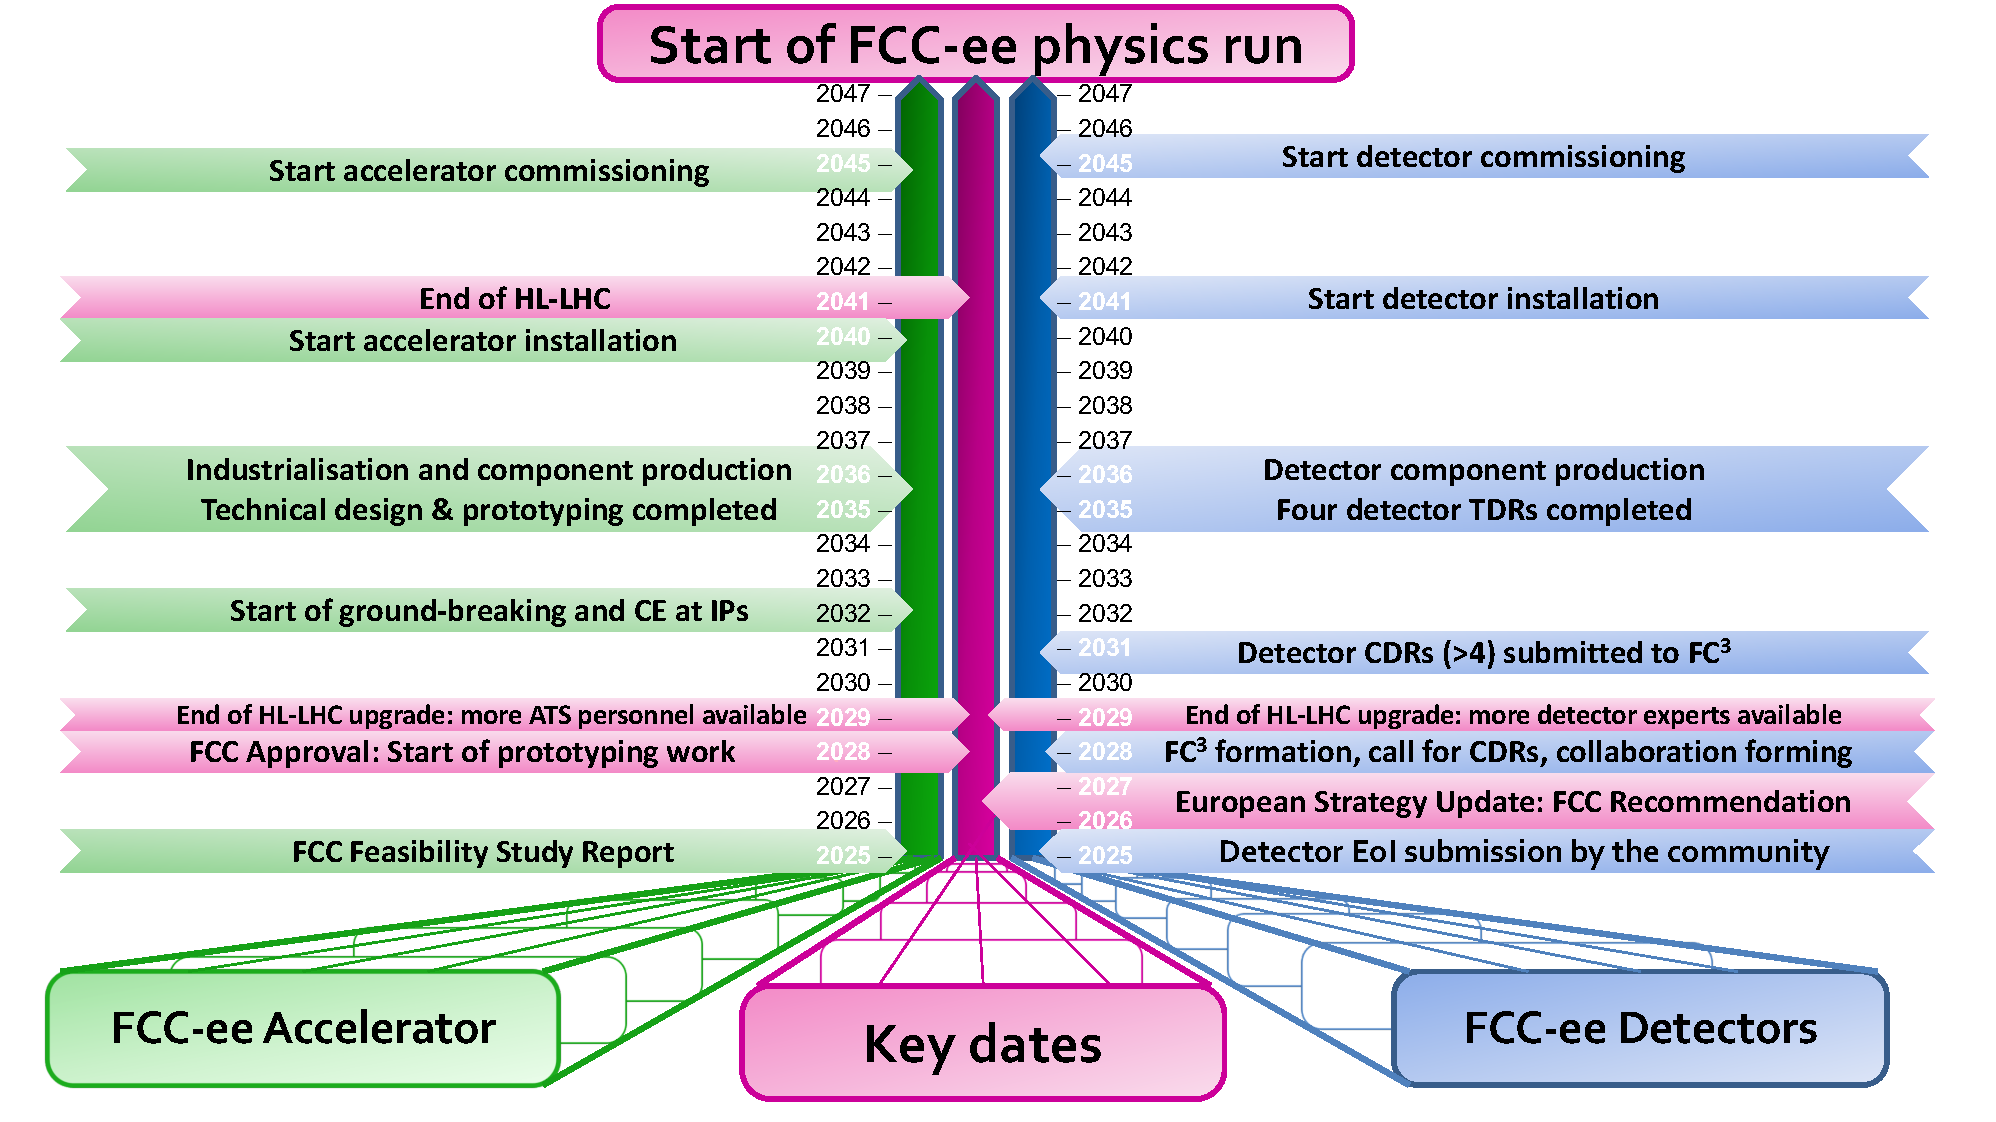
\includegraphics[width=\columnwidth,angle=0]{Outlook/Figs/Roadmap.pdf}
\end{minipage}
\end{sideways}
\end{figure}

The first of these milestones has been for the particle physics community to prepare expressions of interest (EoIs) for critical detector components towards the realisation of up to four experiments, in time for the forthcoming European Strategy Update. More EoIs are foreseen if FCC-ee is recommended as the preferred post-LHC project at CERN by the European Strategy Group. Should the project be approved by CERN Council on the basis of this recommendation, a formal call for the creation of experiment proto-collaborations will be launched, towards the submission of Detector Conceptual Design Reports (CDRs) a few years later, followed by detector Technical Design Reports (TDRs) in the mid-2030's. Achieving these ambitious goals will require an appropriate and timely re-organisation of activities over the coming couple of years, and a significant injection of (human and financial) resources in the project.


In parallel with detector design, construction, installation, and commissioning, the road towards the first collisions is paved with many other exigencies to respond to, a partial list of which follows.  
\begin{itemize}
\item First and foremost, the effort towards the goal of matching theoretical calculation uncertainties to the expected statistical power of the collider (and propagating these calculations to technically accurate Monte Carlo generators), so as to optimally exploit the data from FCC-ee and, later, from FCC-hh, needs to be immediately structured and sustained with appropriate resources, from the clear roadmap established during the Feasibility Study. 

\item In the coming few years, the requirements from detailed physics case studies will continue to be the driving factor in efforts to design the most technologically-advanced (but also the most realistic) FCC-ee detector concepts, to ensure the full coverage of the wide and challenging physics programme. These efforts will have to be intensified, in particular at the \PZ pole, where the requirements from physics are expected to be the most demanding. 

\item These physics studies will need to be backed up with a versatile and reliable software ecosystem, from accurate Monte Carlo event generators to modern event reconstruction and analysis software, passing through detailed detector simulation. Achieving this will demand a significant increase of both computing and human resources, which were a limiting factor during the Feasibility Study. To broaden the project resource base, continued efforts are required to attract (many) more external contributors from institutes worldwide. Promoting positions shared between LHC and FCC will also foster joint development efforts and enhance expertise exchange. 

\item Regarding the interaction region, the integration strategy of the inner sub-detectors (e.g., vertex detectors, luminometers, superconducting pipes, supporting structures) with the accelerator components will be established, as their designs are finalised.   
Methods for opening and maintenance of the detector elements, together with their alignment with respect to the beams will be further developed, and possible consequences on the cavern dimensions will be evaluated. Most importantly, the studies of the impact of all beam-induced backgrounds on the detector performance and mitigation solutions will need to be consolidated for all sub-detectors.

\item The measurement and monitoring of the centre-of-mass energy will be one of the cornerstones of the whole physics programme. The baseline scheme presented in this Volume must be refined and made fully reliable, and alternative schemes will be considered. Specifically, the possibility of injecting already polarised electron and positron bunches will be thoroughly investigated. Improved schemes for monochromatisation will be systematically studied in view of proposing a sustainable method for the electron Yukawa coupling measurement. 

\item Finally, detailed studies of the physics programme of FCC-ee on the one hand, 
and groundwork studies of physics and detectors at FCC-hh on the other, 
will continue to further extend the exploration of the standalone potential of each collider, 
and the synergies between them.
These efforts will also reflect 
the guidelines that will emerge from the review of the Feasibility Study Report and from the ESPPU discussions.

\end{itemize}
While it will be years before all these goals are attained, there is no doubt that the recommendation of the FCC project by the forthcoming ESU will catalyse the engagement of the particle physics community at large on FCC-ee. The growing interest from young scientists in the project must be recognised with appropriate career opportunities.

The baseline choice of collision energies and running sequence (\PZ pole, $\PW\PW$ threshold, $\PZ\PH$ maximum, and $\ttbar$ threshold, as shown in Fig.~\ref{fig:cdrplus}) with four interaction points is sufficient to demonstrate that FCC-ee offers an extraordinary list of opportunities (and associated challenges) for milestone measurements with a real chance of discovery. Looking ahead, this list will only become richer as the investigations deepen, and it is already clear that more integrated luminosity and the extension of the programme to encompass additional energy points would increase the FCC science value still further~\cite{note-FCCeeSequence}. In parallel, the FCC-ee machine parameters are now  different from  those that prevailed at the time of the CDR, and will continue to evolve in the next phase of the study, while the  understanding of the  physics performance of the experiments is progressing. This perspective may significantly modify, or enrich, the desirable scientific programme, as pictured in Fig.~\ref{fig:cdrplus}.

\begin{figure}[htbp]
\centering
\begin{sideways}
\begin{minipage}{175mm} 
\caption{\label{fig:cdrplus} 
Potential physics programme for FCC-ee, ordered by increasing centre-of-mass energy, without indication of a specific chronological sequence. The events highlighted in red indicate the minimal programme with fifteen years of running, and with the corresponding integrated luminosities and physics outcome. The numbers of \PZ, $\PW\PW$, $\PZ\PH$, and $\ttbar$ events delivered to four interaction points are indicated.  A possible wider physics programme, with additional centre-of-mass energies, is highlighted in blue.}
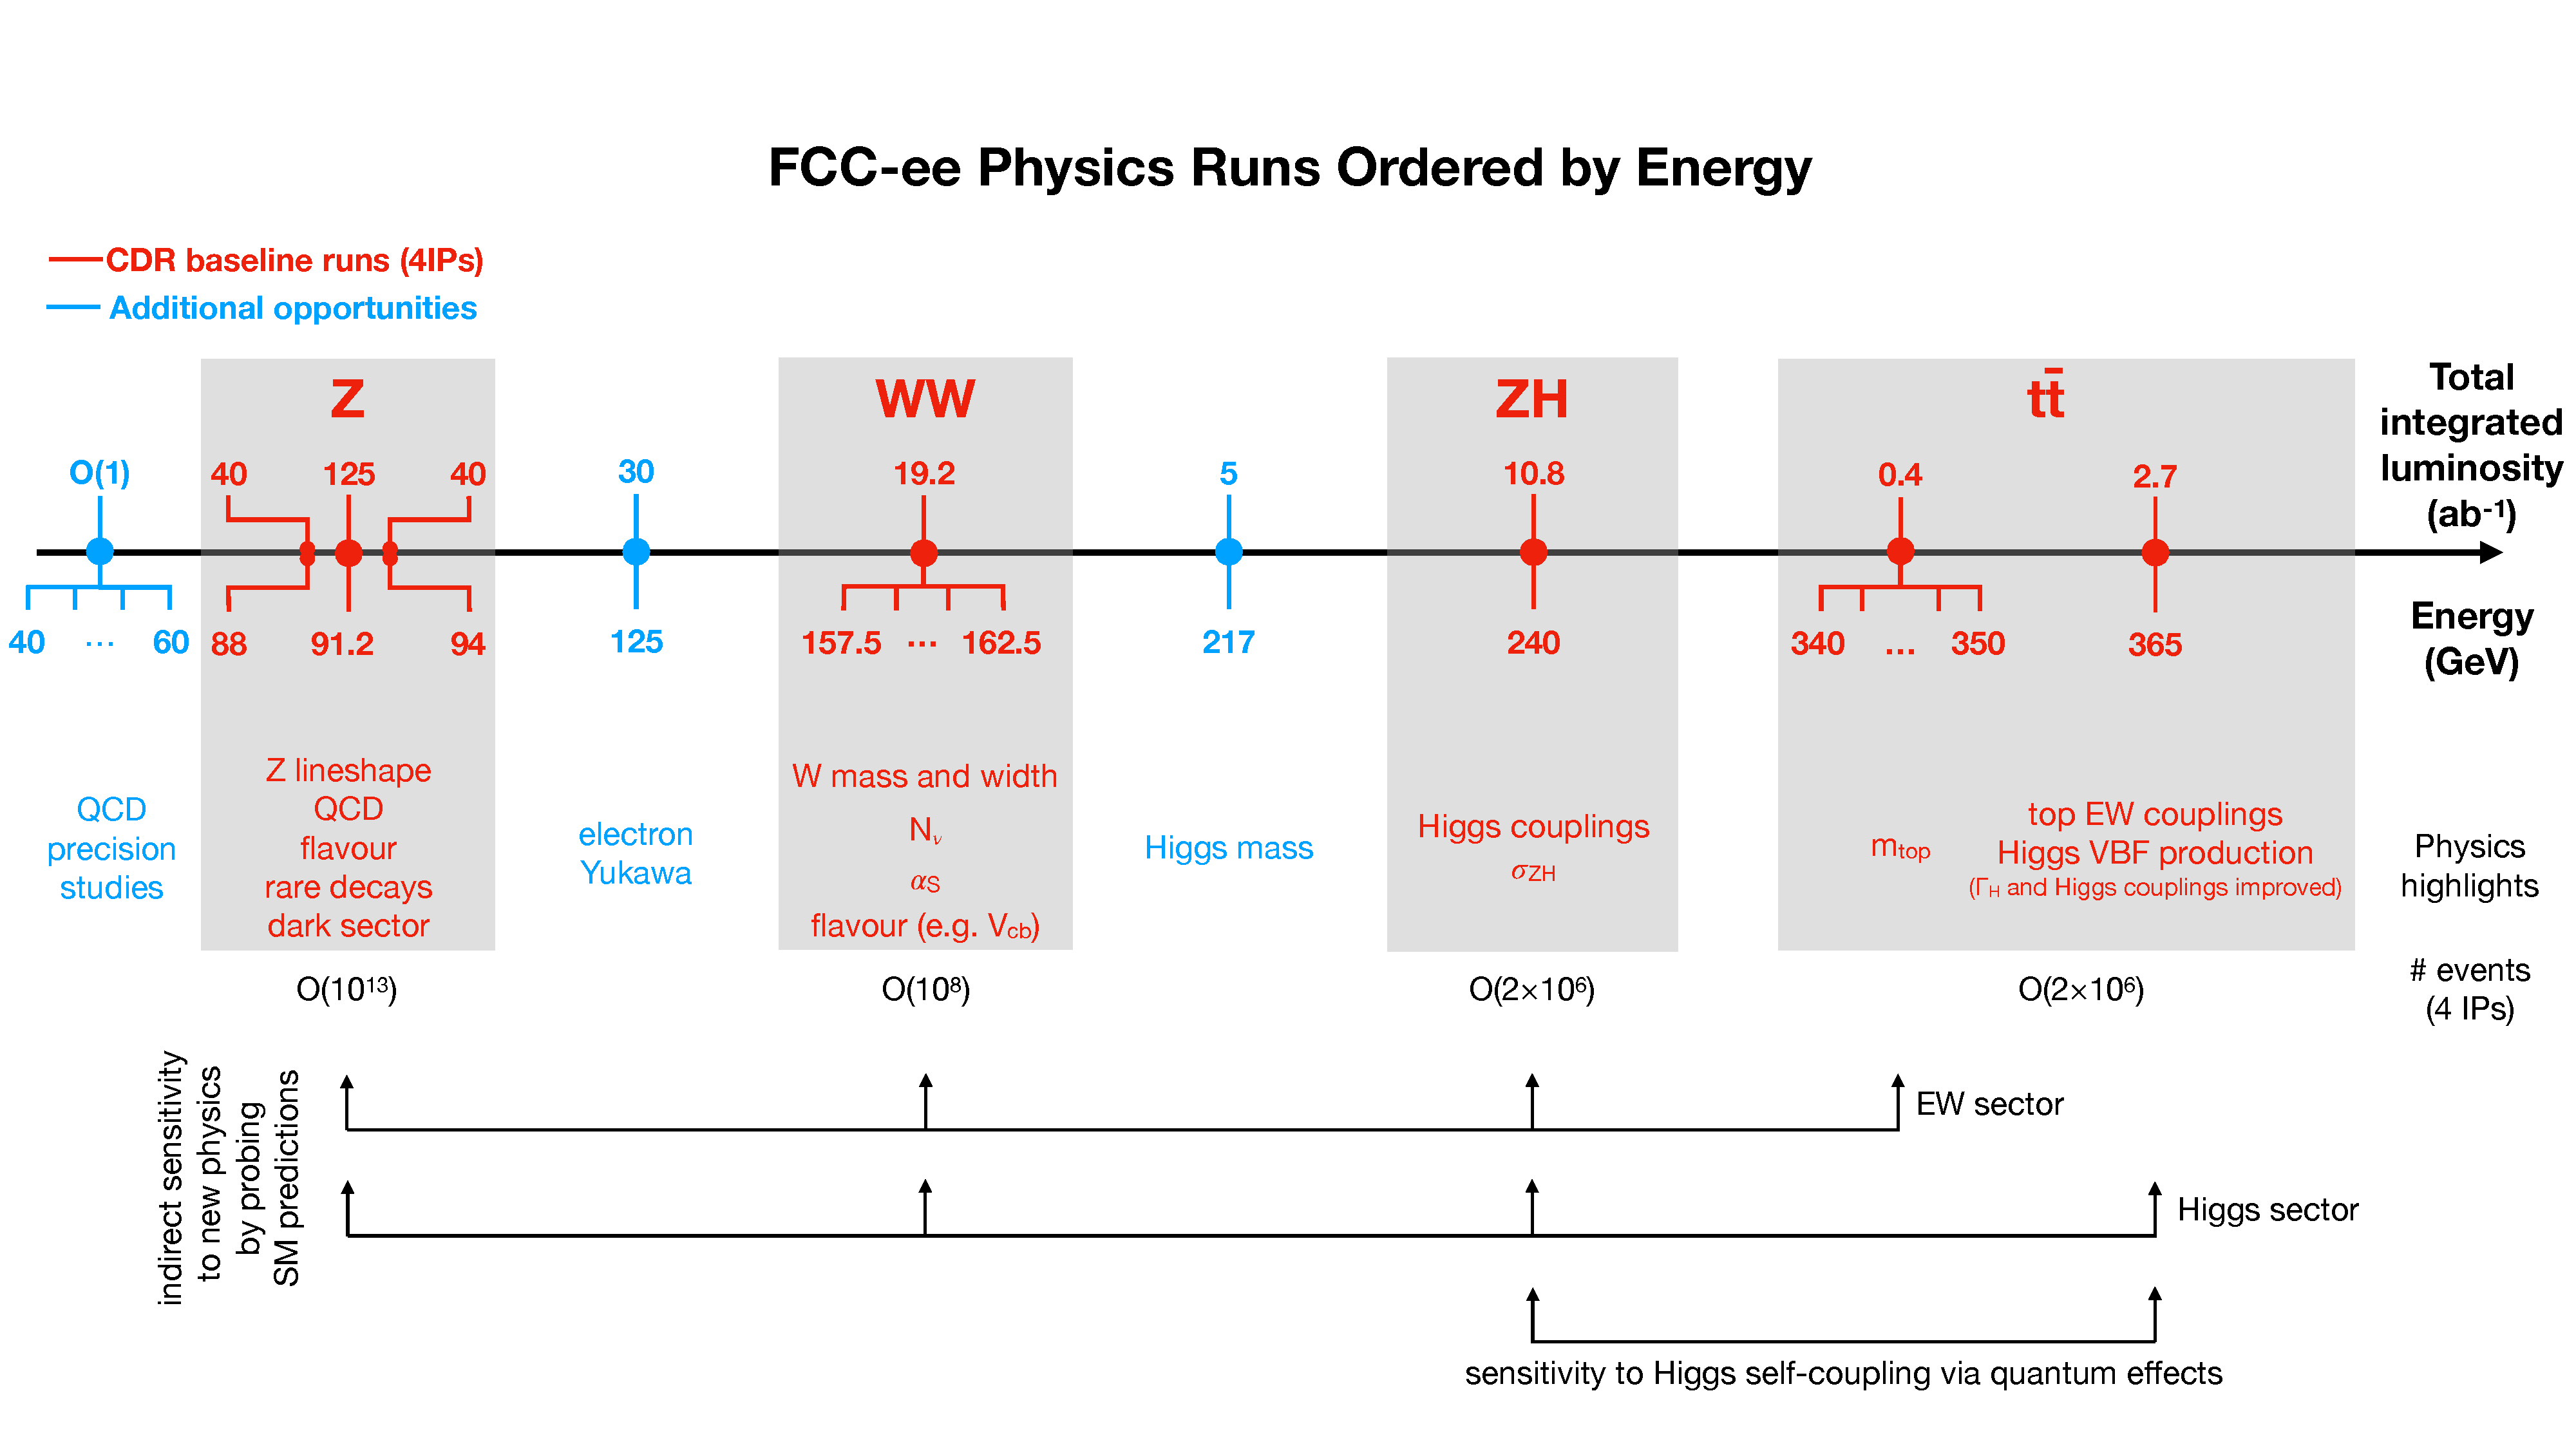
\includegraphics[width=\columnwidth,angle=0]{Physics/Outlook/Figs/FCC-runs.pdf}
\end{minipage}
\end{sideways}
\end{figure}

For example, the possibility to run at $\sqrt{s} = 125$\,GeV, with a centre-of-mass energy spread of the order of the Higgs boson width, is under consideration, towards a 3\,$\sigma$ evidence for the electron Yukawa coupling. Precision QCD studies with a few ab$^{-1}$ at centre-of-mass energies of 20, 30, 40, \dots, 80\,GeV are very appealing to a significant fraction of the HEP community. Because the study of the  monochromatisation schemes required for the electron Yukawa measurement are not yet at a mature stage; and because $\PZ$-pole data with energetic initial-state radiation can in principle also explore lower centre-of-mass energies; no proposal is made yet to include these energy points in the baseline programme. 

These additional possibilities and corresponding science value further demonstrates the flexibility and breadth of the FCC-ee physics potential. An increase of the FCC-ee specific luminosity would enable the physics programme to be extended to encompass at least some of these possibilities within the currently envisaged 15-year timescale. It will ultimately be up to the experimental collaborations and the relevant scientific committees to optimise the time flexibility and to tailor the FCC-ee operation scenario according to a number of factors that cannot be controlled today. For example, external events such as the FCC-hh magnet readiness or the CERN financial situation may call for a change in the overall duration of the FCC-ee running time. Furthermore, intriguing early results may motivate additional running at a given working  point. Meanwhile, new avenues will be explored towards increasing the luminosities at all energies.

At the end of the HL-LHC operation, 
the LEP-LHC integrated programme will have delivered sustained scientific excellence for over 50 years, and greatly advanced our understanding of the fundamental interactions.   The succession of FCC-ee and FCC-hh in a common tunnel will replicate and magnify this success, with vastly better precision and increased energies. The FCC integrated programme offers outstanding prospects for progress in a wealth of topics, including Higgs, electroweak, and flavour physics, as well as remarkable sensitivity in direct searches for both feebly coupled low-mass particles and those that may exist up to many tens of TeV. The upcoming ESPPU provides an opportunity for the global HEP community to endorse this vision, and then to work together so as to enable the first stage of this project, FCC-ee, to be realised in a timely fashion. Seizing this opportunity will be an important step forward in the journey towards a more complete understanding of the laws of nature.   